% 2010 年北京卷理科第 8 题：正方体 ABCD-A1B1C1D1，E、F 在 A1B1 上，P 在 AD，Q 为 CD 中点。
% 来源 PDF：普通高考/2010/2010北京理.pdf，SHA-256 6b5819672aaf59aecfce92e08c2d045a80575803527d61813497dd669a8d5529。
% 原页：第 1 页（A3 三栏）第 2 栏上部，书页码 575。
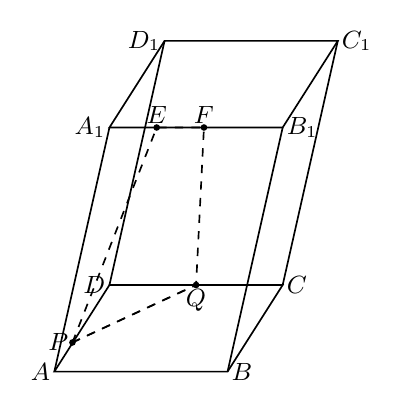
\begin{tikzpicture}[semithick, every node/.style={inner sep=1.2pt, font=\small}]
  \coordinate (A) at (0,0);
  \coordinate (B) at (2.2,0);
  \coordinate (C) at (2.9,1.1);
  \coordinate (D) at (0.7,1.1);
  \coordinate (A1) at (0.7,3.1);
  \coordinate (B1) at (2.9,3.1);
  \coordinate (C1) at (3.6,4.2);
  \coordinate (D1) at (1.4,4.2);
  % 可见棱
  \draw (A) -- (B) -- (C) -- (D) -- cycle;
  \draw (A) -- (A1);
  \draw (B) -- (B1);
  \draw (C) -- (C1);
  \draw (D) -- (D1);
  \draw (A1) -- (B1) -- (C1) -- (D1) -- cycle;
  % E、F 在 A1B1 上
  \coordinate (E) at (1.3,3.1);
  \coordinate (F) at (1.9,3.1);
  % P 在 AD 上，Q 为 CD 中点
  \coordinate (P) at (0.23,0.37);
  \coordinate (Q) at (1.8,1.1);
  \fill (E) circle (1.2pt);
  \fill (F) circle (1.2pt);
  \fill (P) circle (1.2pt);
  \fill (Q) circle (1.2pt);
  \draw[dashed] (P) -- (E) -- (F) -- (Q) -- cycle;
  \draw[dashed] (P) -- (Q);
  % 标注
  \node[left] at (A) {$A$};
  \node[right] at (B) {$B$};
  \node[right] at (C) {$C$};
  \node[left] at (D) {$D$};
  \node[left] at (A1) {$A_1$};
  \node[right] at (B1) {$B_1$};
  \node[right] at (C1) {$C_1$};
  \node[left] at (D1) {$D_1$};
  \node[above] at (E) {$E$};
  \node[above] at (F) {$F$};
  \node[left] at (P) {$P$};
  \node[below] at (Q) {$Q$};
\end{tikzpicture}
